% !TeX spellcheck = es_ES
%----------------------------------------------------------------------------------------
%	PACKAGES AND OTHER DOCUMENT CONFIGURATIONS
%----------------------------------------------------------------------------------------

\documentclass[fleqn,10pt]{SelfArx} % Document font size and equations flushed left
%\usepackage{chemmacros}
\usepackage{ifthen}
\usepackage{calc}
\usepackage{microtype}
\usepackage{ifpdf}
\usepackage[utf8]{inputenc}
\usepackage{amsmath, amsfonts, amssymb}
\usepackage{graphicx, xcolor}
\usepackage{booktabs}
\usepackage{fancyhdr}
\usepackage{lastpage}
\usepackage{titlesec}
\usepackage{titletoc}
\usepackage{enumitem}
%\usepackage{cuted}
\usepackage[version=3]{mhchem}
\usepackage{graphbox}
\usepackage{tabularx}
%----------------------------------------------------------------------------------------
%	COLUMNS
%----------------------------------------------------------------------------------------

\setlength{\columnsep}{0.55cm} % Distance between the two columns of text
\setlength{\fboxrule}{1pt} % Width of the border around the abstract

%----------------------------------------------------------------------------------------
%	COLORS
%----------------------------------------------------------------------------------------

\definecolor{color1}{RGB}{0,94,157} % Color of the article title and sections
\definecolor{color2}{RGB}{255,243,210} % Color of the boxes behind the abstract and headings

%----------------------------------------------------------------------------------------
%	HYPERLINKS
%----------------------------------------------------------------------------------------

\usepackage{hyperref} % Required for hyperlinks
\hypersetup{hidelinks,colorlinks,breaklinks=true,urlcolor=color2,citecolor=color1,linkcolor=color1,bookmarksopen=false,pdftitle={Title},pdfauthor={Author}}

%----------------------------------------------------------------------------------------
%	ARTICLE INFORMATION
%----------------------------------------------------------------------------------------

\JournalInfo{L. de Qu\'imica inorg\'anica II, No. 7, 2016-20} % Journal information
%\Archive{Additional note} % Additional notes (e.g. copyright, DOI, review/research article)

\PaperTitle{La constante de estabilidad del \ce{Ni(Gly^-)_n^{(2-n)+}}} % Article title

\Authors{Juan Barbosa{\color{color1}\textsuperscript{1}\textsuperscript{,2}*},
	Alejandro Camacho{\color{color1}\textsuperscript{1}\textsuperscript{,3}**}} %
%Authors
\affiliation{{\color{color1}\textsuperscript{1}}\textit{Departamento de Qu\'imica, Universidad de los Andes, Bogot\'a, Colombia}} % Author affiliation
\affiliation{{\color{color1}\textsuperscript{2}}\textit{Departamento de F\'isica, Universidad de los Andes, Bogot\'a, Colombia}} % Author affiliation
\affiliation{{\color{color1}\textsuperscript{3}}\textit{Departamento de	F\'isica, Universidad Nacional, Bogot\'a, Colombia}}
\affiliation{{\color{color1}*}\textbf{Email}: js.barbosa10@uniandes.edu.co} %
%Corresponding author
\affiliation{{\color{color1}**}\textbf{Email}: a.camacho10@uniandes.edu.co}
\Keywords{amino\'acidos, glicina, bioinorg\'anica, constantes de estabilidad} %
%Keywords - if you don't want any simply remove all the text between the curly
%brackets
\newcommand{\keywordname}{Keywords} % Defines the keywords heading name

%----------------------------------------------------------------------------------------
%	ABSTRACT
%----------------------------------------------------------------------------------------
\Abstract
{
}
%----------------------------------------------------------------------------------------

\begin{document}
	\flushbottom % Makes all text pages the same height
	\maketitle % Print the title and abstract box
	%\tableofcontents % Print the contents section
	\thispagestyle{empty} % Removes page numbering from the first page
	%----------------------------------------------------------------------------------------
	%	ARTICLE CONTENTS
	%----------------------------------------------------------------------------------------
	\section*{Introducci\'on}	
	La glicina es un amino\'acido cuya funci\'on es la de un inhibidor de funciones neurotransmisoras en la esp\'ina dorsal, y retina \cite{Glycine}. Fue descubierta en 1820 por Henri Braconnot cuando realizaba experimentos con gelatina y \'acido sulf\'urico. Actualmente hace parte de los 21 amino\'acidos esenciales, siendo el \'unico que no presenta quiralidad \cite{GlycineHistory}.
	\begin{scheme}[h]
	   	\centering
	   	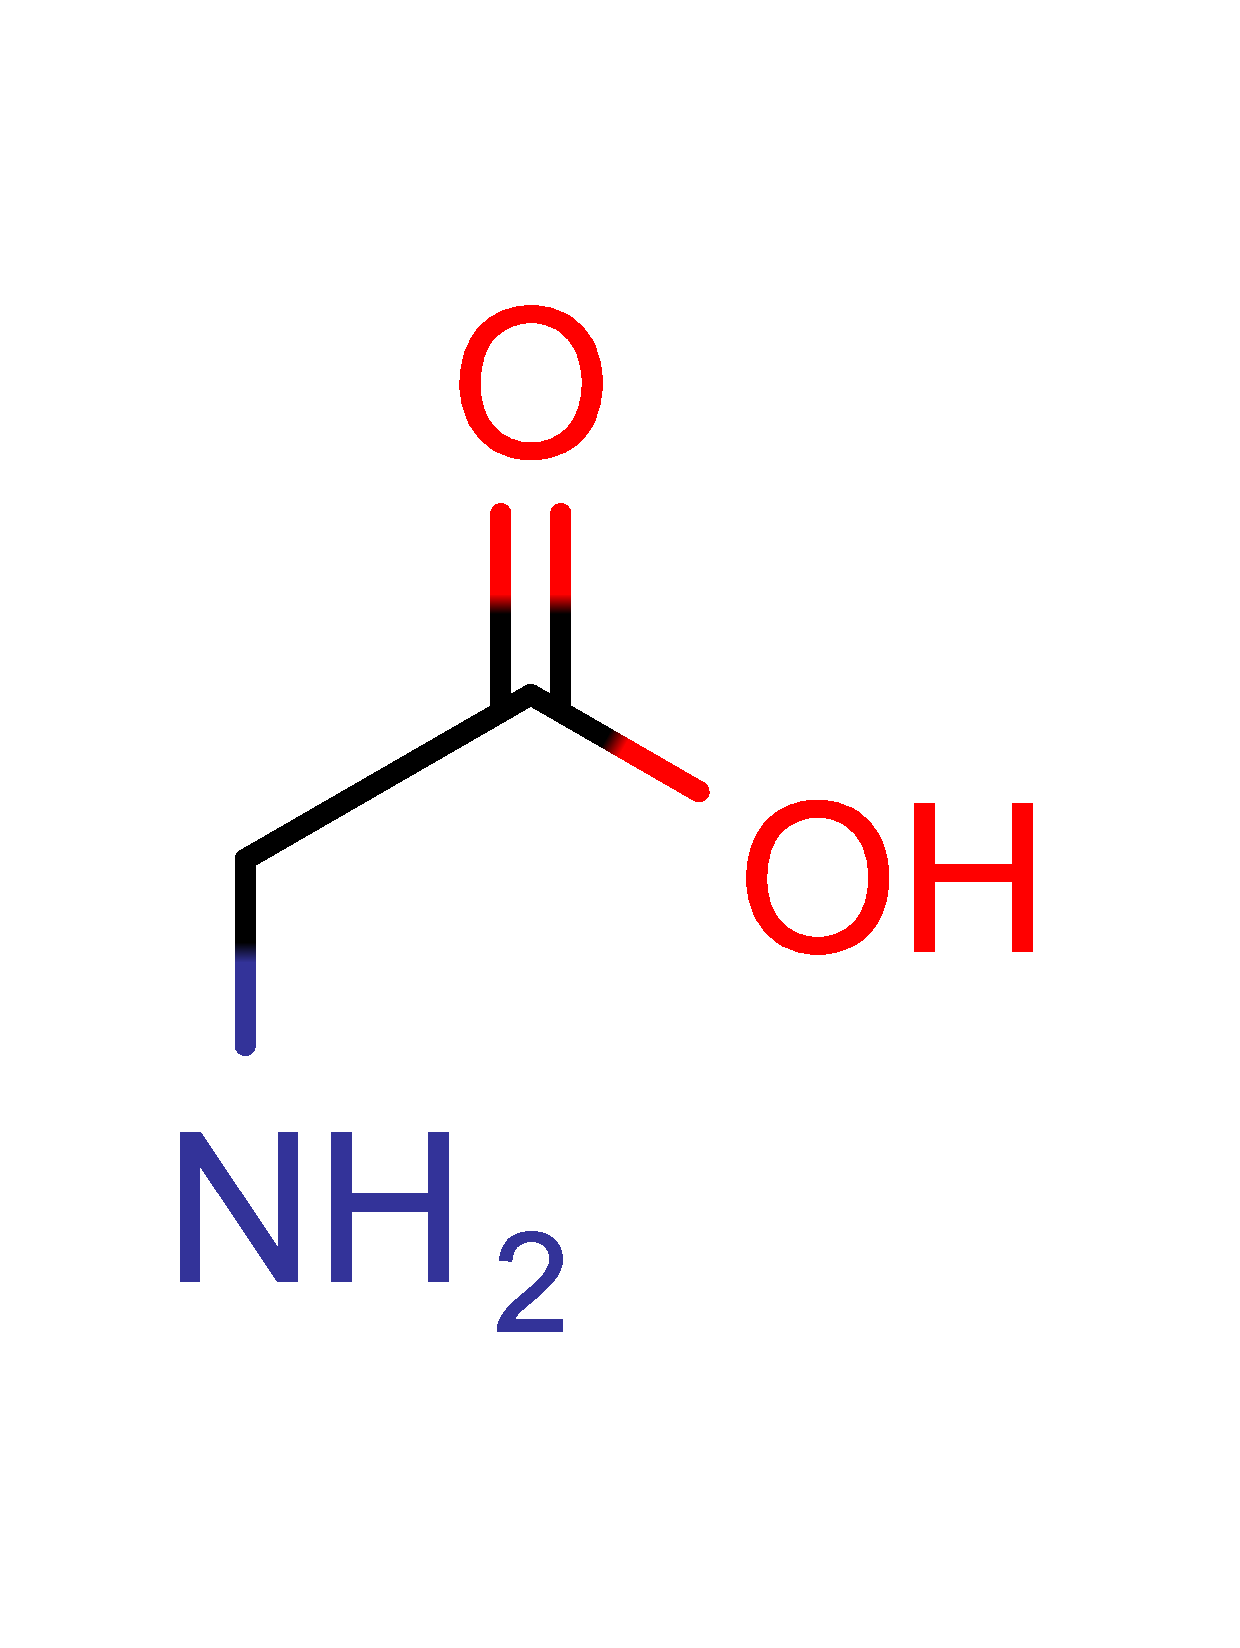
\includegraphics[width=0.3\linewidth]{images/Glicina}
	   	\caption{Estructura qu\'imica de la glicina.}
	   	\label{fig:glicina}
	\end{scheme}
	
	La bioinorg\'anica del n\'iquel tambi\'en tiene sus pecularidades, dado que fue el \'unico metal de transici\'on con periodo 3 al que no se le hab\'ian atribu\'ido funciones biol\'ogicas para 1975. Lo anterior se debi\'o en parte a que el n\'iquel no presenta bandas de absorci\'on caracter\'isticas al coordinarse con ligandos biol\'ogicos. La perspectiva biol\'ogica del n\'iquel cambi\'o al descubrirse que la ureasa es una enzima de este metal \cite{Nickel}. 
    
    En general, el n\'iquel al igual que la mayor\'ia de metales de transici\'on prefiere una geometr\'ia tetra\'edrica. Por esta raz\'on se tiene un n\'umero m\'aximo de coordinaci\'on 6, sin embargo como el glicinato act\'ua como un ligando bidentado, es posible alcanzar \'unicamente tres diferentes iones en soluci\'on con constantes de equil\'ibrio $K_1$, $K_2$ y $K_3$, los cuales se muestran en la \autoref{fig:ligands}:    
    \footnotesize
    \begin{equation*}
        \begin{array}{cc}
        \ce{Ni^{2+} + Gly- <=> Ni(Gly)+} & K_1 = \dfrac{\ce{[Ni(Gly)+]}}{\ce{[Ni^{2+}][Gly^-]}}\\
        \ce{Ni(Gly)+ + Gly- <=> Ni(Gly)_2} & K_2 = \dfrac{\ce{[Ni(Gly)_2]}}{\ce{[Ni(Gly)+][Gly^-]}}\\
        \ce{Ni(Gly)_2 + Gly- <=> Ni(Gly)_3-} & K_3 = \dfrac{\ce{[Ni(Gly)_3^-]}}{\ce{[Ni(Gly)_2][Gly^-]}}
        \end{array}
    \end{equation*}
    \normalsize
    
    Con el objetivo de facilitar los c\'alculos posteriores se introducen las constantes de equilibrio globales:
    \begin{equation}
	    \beta_n = \prod\limits_{i=1}^{i \leq n} K_i
    \end{equation}
    
    Usando el m\'etodo de J. Bjerrum es posible calcular las constantes globales conociendo la relaci\'on entre las moles de glicinato ligado y el cati\'on libre.
    \small  
    \begin{equation}
    \def\arraystretch{3}
	    \begin{array}{rl}
		    \tilde{n} & = \dfrac{\ce{\beta_1[Gly^-] + 2\beta_2[Gly^-]^2 + 3\beta_3[Gly^-]^3}}{\ce{1 + \beta_1[Gly^-] + \beta_2[Gly^-]^2 + \beta_3[Gly^-]^3}} \\
		    & = \dfrac{\ce{[Gly]}_0 - (1+K_a/\ce{[H+]})(C_H + \ce{[OH^-] - [H+]})}{\ce{[NiCl2]}_0}
	    \end{array}
    \end{equation}
    \normalsize
    
    Donde $K_a$ es la constante de acidez de la glicina, $C_H$ la concentraci\'on de protones debido al \'acido n\'itrico, y el factor $K_a/\ce{[H+]}(\cdots)$ corresponde con la concentraci\'on de glicina libre \ce{[Gly^-]}. Reescribiendo la ecuaci\'on se obtiene:
    \footnotesize
    \begin{equation}
	    \dfrac{\tilde{n}}{(1-\tilde{n})\ce{[Gly^-]}} = \beta_1 + \dfrac{(2-\tilde{n})}{(1-\tilde{n})}\ce{[Gly^-]}\beta_2 + \dfrac{(3-\tilde{n})}{(1-\tilde{n})}\ce{[Gly^-]}^2\beta_3
    \end{equation}
    \normalsize
    
    Para la realizaci\'on del an\'alisis se toman dos aproximaciones importantes. En primer lugar el coeficiente de actividad $\gamma$ se asume constante a lo largo del experimento dado que la contribuci\'on de los iones distintos al nitrato es despreciable, pues estos u\'ltimos se trabajan con al menos tres \'ordenes de magnitud menos.
    \begin{equation}
	    \ce{[H+]} = \dfrac{10^{-pH}}{\gamma_\pm}
    \end{equation}
    
    En segundo lugar las concentraciones iniciales de glicinato y n\'iquel se asumen constantes a lo largo del experimento, esto debido a que el cambio neto de volumen no supera el 5 \% del volumen inicial.
    \begin{figure*}[h]
    	\centering
    	\begin{tabular}{ccc}
    		\includegraphics[width=0.2\linewidth]{images/Single.png} & \includegraphics[width=0.4\linewidth]{images/Double.png} &
    		\includegraphics[width=0.3\linewidth]{images/Triple.png}
    	\end{tabular}
    	\caption{Distintos complejos de glicinato de n\'iquel en soluci\'on. Las esf\'eras rojas representan ox\'igenos, en gris se muestran los carbonos, hidr\'ogenos en blanco, y los \'atomos de nitr\'ogeno en azul.}
    	\label{fig:ligands}
    \end{figure*}
	\section{Metodolog\'ia}

	\section{Resultados y Discusi\'on}
	Con el objetivo de obtener un valor estimado para la constante de acidez de la glicina se llev\'o a cabo una simulaci\'on de protonaci\'on sobre la mol\'ecula. Con lo cual se obtuvieron 71 puntos que posteriormente fueron usados en una interpolaci\'on c\'ubica con el objetivo de encontrar el valor de pH para el cual el porcentaje de formaci\'on corresponde con 50 \%. Los datos obtenidos de la simulaci\'on con Marvin y el algoritm\'o de interpolaci\'on se encuentran disponibles en \href{www}{text}
	\begin{figure}[h]
		\centering
		\includegraphics[width=\linewidth]{images/pka_sim.pdf}
		\caption{Simulaci\'on de la constante de acidez de la glicina.}
	\end{figure}
	
	\section{Preguntas}
	\subsection{Dibujar todos los is\'omeros \'opticos y geom\'etricos de los tres complejos de}
	\subsubsection{\ce{[Ni(Gly^-)]^+}}
	\subsubsection{\ce{[Ni(Gly^-)_2]}}
	\subsubsection{\ce{[Ni(Gly^-)]_3^-}}
	
	\subsection{Derivar la ecuaci\'on 11}
	La glicina se deprotona dando lugar a la siguiente reacci\'on:
	\begin{equation}\label{Ka}
	\begin{array}{lr}
	\ce{Gly ->[K_a] H+ + Gly^-} & K_a = \dfrac{\ce{[H+][Gly^-]}}{\ce{[Gly]}}
	\end{array}
	\end{equation}
	
	Aplicando logaritmo a ambos lados y multiplicando por -1 es obtiene una ecuaci\'on para el $pKa$.
	\begin{equation}\label{pKa}
	pK_a = -\log K_a = -\log\ce{[H+]} - \log\left(\dfrac{\ce{[Gly^-]}}{\ce{[Gly]}}\right)
	\end{equation}
	
	Considerando la conservaci\'on de carga en la soluci\'on:
	\begin{equation}
		\ce{[Gly^-]} = \ce{[H+] + [Na+] - [OH^-]}
	\end{equation}
	
	Aplicando conservaci\'on de la masa:
	\footnotesize
	\begin{equation}
		\ce{[Gly]} = \ce{[Gly_0]-[Gly^-]} = \ce{[Gly_0]} - \left(\ce{[H+] + [Na+] - [OH^-]}\right)
	\end{equation}
	\normalsize
	
	\small
	Reemplazando las ecuaciones anteriores en la \autoref{pKa}.	
	\begin{equation*}
		pKa = -\log\ce{[H+]} - \log\left(\dfrac{\ce{[H+] + [Na+] - [OH^-]}}{\ce{[Gly_0]} - \left(\ce{[H+] + [Na+] - [OH^-]}\right)}\right)
	\end{equation*}
	\normalsize
	
	\subsection[Se prepara]{Se prepara una disoluci\'on por mezclar de 100 mL de glicina (0.2 M) y 100 mL de \ce{Cu^{2+}} (0.2 M), el pH se ajust\'o a 7 con una soluci\'on de NaOH. Calcule los porcentajes aproximados del ion \ce{Cu^{2+}} original, as\'i como los actuales despu\'es de efectuar la mezcla, \ce{Cu^{2+}}, \ce{CuA+}, y \ce{CuA_2} en la soluci\'on. Use $pK_a$ de 9.60 para la glicina y las siguientes constantes de estabilidad}:
	\begin{equation*}
	    \begin{array}{lcrc}
	        \ce{Cu^{2+} + A-} & \ce{<=>} & \ce{CuA+} & \log K_1 = 8.38\\
	        \ce{CuA+ + A-} & \ce{<=>} & \ce{CuA_2} & \log K_2 = 6.87 
	    \end{array}
	\end{equation*}
	
	\subsection{Se desea determinar las constantes de formaci\'on ($K_1$, $K_2$ y $K_3$) para los complejos de coordinaci\'on de etilendiamina, a \ce{Ni^{2+}} formando los complejos \ce{[Ni(en)]^{2+}}, \ce{[Ni(en)_2]^{2+}}, \ce{[Ni(en)_3]^{2+}}}
	\subsubsection{C\'omo determinar\'ia el primer y segundo $pKa$ de la etilendiamina?}
	\subsubsection{Defina estos dos valores de $pKa$. ?`Cu\'al de los dos ser\'ia el m\'as grande?}
	\subsubsection{Cu\'ales titulaciones realizar\'ia para determinar las constantes de estabilidad $K_1$, $K_2$ y $K_3$? Explique brevemente. El procedimiento difiere de lo utilizado en este experimento?}
	\subsubsection{Qu\'e valor esperar\'ia sea m\'as grande, el de $K_1$ o el de $K_2$?}
	
	\subsection{Considere la coordinaci\'on del ligando tridentado iminodiacetato al ion \ce{Cu^{2+}}. Cuando se agrega la forma monoprotonada del iminodiacetato, a una soluci\'on acuosa de \ce{Cu^{2+}}, se establece r\'apidamente el siguiente equilibrio:}
	\begin{equation}
	    \ce{Cu^{2+} + HA- <=> CuA + H+}
	\end{equation}
	
	\section{Conclusiones}
	
	\phantomsection
	\bibliographystyle{unsrt}
	\begin{thebibliography}{9}
	    \bibitem{Glycine}
	    \textit{Glycine}; Encyclopedic Reference of Genomics and Proteomics in Molecular Medicine; Springer Berlin Heidelberg: Berlin. Heidelberg, 2006; pp 703.
	    \bibitem{GlycineHistory}
	    \textit{Glycine}; Encyclopedia of Astrobiology; Springer Berlin Heidelberg: Berlin. Heidelberg, 2015; pp 994.
	    \bibitem{Nickel}
	    Kaim, W.; Schwederski, B.; Klein, A. \textit{Bioinorganic chemistry: Inorganic elements in the chemistry of life - an introduction and guide}, 2nd ed.; Wiley-Blackwell (an imprint of John Wiley \& Sons Ltd): Oxford, United Kingdom, \textbf{2011}; p 300.
	\end{thebibliography}
\end{document}
